\documentclass[12pt]{article}
\usepackage[utf8]{inputenc}
\usepackage{booktabs}
\usepackage{listings}
\usepackage{color}
\usepackage{siunitx}
\usepackage{amsmath}
\usepackage{subcaption}
\usepackage[margin=1in]{geometry}
\usepackage{pgfplots}
\usepackage{tikz}
\usepackage{caption}
\usepackage{subcaption}
\usepackage{algorithm}
\usepackage{algorithmic}
\usepackage{graphicx}

\title{Evolutionary Mechanics}
\author{Tobias Jacob, Raffaele Guillera, Ali Muddasar}

\begin{document}

\maketitle

\begin{abstract}
    We developed an application that is able to develop mechanical structures using an evolutionary algorithm. This approach can be scaled efficiently across many different nodes.
\end{abstract}

\section{Introduction}

With increasing computing power available, a new approach is becomeing more relevant in engineering: Evolutionary algorithms. Instead of developing a structure for a problem, an engineer just specifies the structure of the problem and lets the computer come up with a solution. The hope is that the computer will come up with a better solution the engineer did not think of.

\section{Method}

Our project is divided in two sections and corresponding layers of parallelism. The first one is solving the mechanical equations to check if a mechanical structure can withstand a force. Figure~\ref{fig:Mechanical_Simulation} shows the result of such a simulation. The shape of a figure is approximated through squares. A detailed introduction on how to use the fininte element method can be found at~\cite{Nikishkov2004}. We used \texttt{OpenMP} for this part.

\begin{figure}[h]
    \centering
    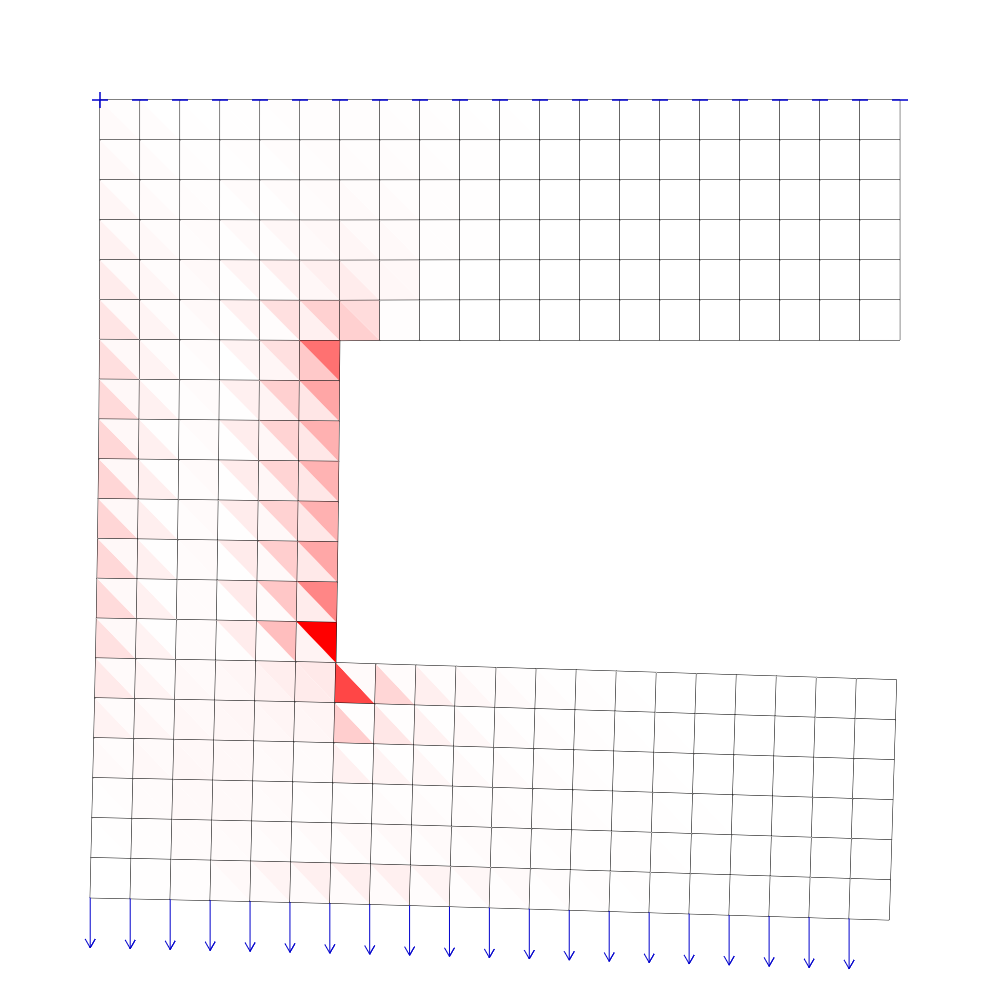
\includegraphics[width=0.5\textwidth, trim={0pt 0pt 0pt 5em}, clip]{images/MechaincalStructure.png}
    \caption{Result of a mechanical simulation}
    \label{fig:Mechanical_Simulation}
\end{figure}


The second stage is the evolutionary algorithm. The best 10\% survive in each round. The structures mutate and are simulated again. We used \texttt{MPI} for this part.

\subsection{Speeding up the equation solver}

\begin{figure}[p]
    \centering
    % This file was created by tikzplotlib v0.9.6.
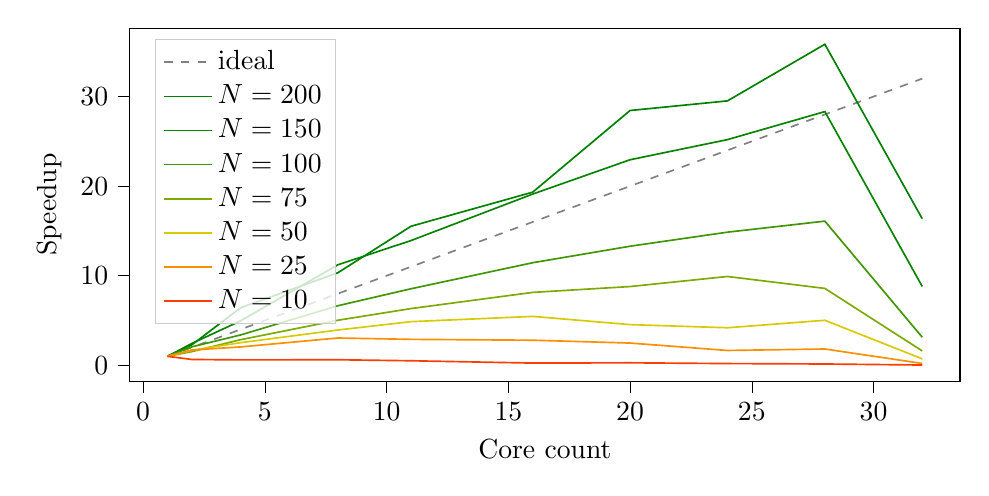
\begin{tikzpicture}

\definecolor{color0}{rgb}{0.0313725490196078,0.512664359861592,0}
\definecolor{color1}{rgb}{0.250980392156863,0.587589388696655,0}
\definecolor{color2}{rgb}{0.486274509803922,0.667866205305652,0}
\definecolor{color3}{rgb}{0.847058823529412,0.790957324106113,0}
\definecolor{color4}{rgb}{1,0.555478662053057,0}
\definecolor{color5}{rgb}{1,0.238062283737024,0}

\begin{axis}[
height=0.5\textwidth,
legend cell align={left},
legend style={fill opacity=0.8, draw opacity=1, text opacity=1, at={(0.03,0.97)}, anchor=north west, draw=white!80!black},
tick align=outside,
tick pos=left,
width=\textwidth,
x grid style={white!69.0196078431373!black},
xlabel={Core count},
xmin=-0.55, xmax=33.55,
xtick style={color=black},
y grid style={white!69.0196078431373!black},
ylabel={Speedup},
ymin=-1.75896654666474, ymax=37.6252733144807,
ytick style={color=black}
]
\addplot [semithick, white!50.1960784313725!black, dashed]
table {%
1 1
2 2
4 4
8 8
11 11
16 16
20 20
24 24
28 28
32 32
};
\addlegendentry{ideal}
\addplot [semithick, green!50.1960784313725!black]
table {%
1 1
2 2.28099772207445
4 6.4213007586338
8 10.33333403677
11 15.5180451413758
16 19.325867308679
20 28.4408787953592
24 29.5148957972303
28 35.8350805935196
32 16.3610316622339
};
\addlegendentry{$N = 200$}
\addplot [semithick, color0]
table {%
1 1
2 2.43816479897117
4 4.95731016621839
8 11.2206829951489
11 13.921817302774
16 19.1127015275694
20 22.9446177937192
24 25.1921540782817
28 28.3185033472583
32 8.80166918432349
};
\addlegendentry{$N = 150$}
\addplot [semithick, color1]
table {%
1 1
2 2.06085823640149
4 3.38683240554257
8 6.65048670634881
11 8.54275031459705
16 11.4503068589557
20 13.2921764372414
24 14.8616137051205
28 16.0915338713289
32 3.13487450337091
};
\addlegendentry{$N = 100$}
\addplot [semithick, color2]
table {%
1 1
2 1.52890912153782
4 2.85800715096875
8 5.03039692757545
11 6.33346520726186
16 8.13838875944362
20 8.7912624321191
24 9.91441522806836
28 8.58340718014402
32 1.60447891045102
};
\addlegendentry{$N = 75$}
\addplot [semithick, color3]
table {%
1 1
2 1.67986100619429
4 2.52454549877556
8 3.94170971335967
11 4.87049841994931
16 5.46033639090096
20 4.54214142946763
24 4.19104799084607
28 5.02464453446523
32 0.720257443013434
};
\addlegendentry{$N = 50$}
\addplot [semithick, color4]
table {%
1 1
2 1.70629980573286
4 2.05167564475378
8 3.04823287768256
11 2.89759644516259
16 2.80122363967717
20 2.48472951908088
24 1.65639071700727
28 1.8207894402843
32 0.205706911385145
};
\addlegendentry{$N = 25$}
\addplot [semithick, color5]
table {%
1 1
2 0.652204015693515
4 0.602815699658703
8 0.61946514686541
11 0.507451966241695
16 0.248899066408314
20 0.278478517934568
24 0.194936883493137
28 0.14711087975013
32 0.0312261742964166
};
\addlegendentry{$N = 10$}
\end{axis}

\end{tikzpicture}

    \caption{Speedup of the equation solver for different proplem sizes $N$.}
    \label{fig:SpeedupSimulation}
\end{figure}

\begin{table}[p]
    \centering
    \begin{tabular}{lrrrrrrr}
\toprule
{} & $N = 10$ & $N = 25$ & $N = 50$ & $N = 75$ & $N = 100$ & $N = 150$ & $N = 200$ \\
\midrule
Problem size &      230 &     1325 &     5150 &    11475 &     20300 &     45450 &     80600 \\
\midrule
1            &        3 &       43 &      311 &     1153 &      3306 &     19869 &     97932 \\
2            &        4 &       25 &      185 &      754 &      1604 &      8149 &     42934 \\
4            &        5 &       21 &      123 &      403 &       976 &      4008 &     15251 \\
8            &        5 &       14 &       79 &      229 &       497 &      1771 &      9477 \\
11           &        6 &       15 &       64 &      182 &       387 &      1427 &      6311 \\
16           &       11 &       15 &       57 &      142 &       289 &      1040 &      5067 \\
20           &       10 &       17 &       69 &      131 &       249 &       866 &      3443 \\
24           &       14 &       26 &       74 &      116 &       222 &       789 &      3318 \\
28           &       19 &       24 &       62 &      134 &       205 &       702 &      2733 \\
32           &       91 &      209 &      432 &      718 &      1055 &      2257 &      5986 \\
\bottomrule
\end{tabular}
    \caption{Execution time for the equation solver for different field sizes $N$ and cores $C$}
    \label{tab:SpeedupSimulation}
\end{table}

\begin{algorithm}[p]
    \caption{Simulate}
    \begin{algorithmic}
        \STATE Setup the equation system
        \STATE Solve the equation system with the conjugate gradient method
        \STATE Calculate the stress using the Van-Mieses-Equation
    \end{algorithmic}
    \label{alg:Simulation}
\end{algorithm}

The reason for using \texttt{OpenMP} is the tight coupling between the data in the sparse matrix multiplication. \texttt{gprof} revealed that the equation solver spends most of it's time in the sparse matrix multiplication, however the whole equation solver class works parallelized. The concept of the simulation is visualized in algorithm~\ref{alg:Simulation}.

\begin{itemize}
    \item \textbf{Threads are spawned at the highest level} of the \texttt{PerformanceEvaluator} class. Subsequent calls to the equation setup, equation solver or linear algrabra operations will not spawn new threads. They require the threads to be set up already, and process only their their chunk using the \texttt{omp for} directive. All for loops are executed in chunks to \textbf{prevent false sharing}.
    \item The \textbf{equation setup} process adds the local element stiffness matrix into the global equation system. Depending on the mechanical structure, the position of different planes appears rather random. Therefore, a lock is needed to prevent a race condition. Because the matrix is sparse and each thread works on its own plane, that typically are not directly connected, it is unprobable that two threads operate on the same equation row at the same time. A global lock would introduce an unnecessary penalty, therefore each row uses it's own \textbf{lock}.
    \item \textbf{All linear algebra operations of the equation solver work in parallel}, we can divide these in two types:
    
    For addition, scalar multiplication, matrix multiplication or assigning a constant value, each thread processes its \textbf{own chunk of rows}. These operations do not require an implicit or explicit barrier. If for example, a vector addition follows a scalar multiplication, it is fine if the first thread begins with the scalar multiplication before the second thread has finished the vector addition, since each of them operates on its own set of rows.
    
    However, in the conjugate gradient method there are also operations like the scalar product or the norm of the vector. These operations require a \textbf{reduction} and have an implicit barrier.
    \item In the beginning, a unique index has to be assigned to each Plane and corner. This is not parallelizable, as the total number of planes and corners is unkown and does not follow a predictable pattern.
    \item Using the \textbf{conjuage gradient method} reduced the time complexity by $O(N)$~\cite{ProgressReport}.
    \item Using a \textbf{sparse matrix multiplication} reduced the the time complexity by $O(N^2)$~\cite{ProgressReport}. 
\end{itemize}

The time complexity of the sequential equation solver is dominated by the sparse matrix multiplication, having a complexity of 

\begin{equation}
    O_\mathit{seqSolve}(N) = O(N^3) 
\end{equation}

as explained in the progress report~\cite{ProgressReport}. The sparse matrix multiplication has been fully parallelized. The indexing of the equation requires $O(N^2)$. Leaving the overhead for thread creation aside, the runtime complexity is 

\begin{equation}
    O_\mathit{parSolve}(N, C) = O \left(\frac{N^3}{C}\right) + O(N^2)
\end{equation}

for a sufficiently large $N$. The efficency is

\begin{equation}
    E = \frac{O_\mathit{seqSolve}}{O_\mathit{parSolve} C} = O\left(\frac{N^3}{N^3 + C^2}\right)
\end{equation}

As the efficency remains only if $N \propto C$, we can asses that the equation solver has Weak Scalibality. However, there is a significant overhead due to creating the threads. The speedup becomes only notable for problem sizes $N > 100$.

The Equation Solver is still a powerful solver. It is able to solve a mechanical structure with 80600 equations in \SI{2.732}{\second} using 28 cores on bridges. It also showcases OpenMP and locks well. The speedup of the execution time of table~\ref{fig:SpeedupSimulation} are shown in figure~\ref{tab:SpeedupSimulation}.

\subsection{Speeding up the evolutionary algorithm}

Evolutionary algoirthms are easily parallelizable by nature. Each organism can be evaluated independently by each node, while the results will be gathered by a single node in charge of sorting them. The best 10\% get broadcasted to the other nodes again. This is visualized in algorithm~\ref{alg:Evolution}.

A MPI Message for an evaluated board consisits of

\begin{itemize}
    \item 1 float for the score
    \item $R \times C$ bytes, each containing the boolean value of the field.
\end{itemize}

We typically simulate grid sizes of 20, meaning the message has a size of 404 bytes. Since all processes will be initialized with the same field size it has not to be stored in the message. The message size grows with 

\begin{equation}
    O_{msgSize} = O(N^2)
\end{equation}

The runtime complexity of the single thread evolutionary algorithm is

\begin{equation}
    O_\mathit{evolSeq}(N, G, A) = O_\textit{seqSolve} \cdot O(G A)
\end{equation}

with generations size $G$ and $A$ epochs. The parallel version has

\begin{equation}
    O_\mathit{evolPar}(N, C, G, A) = O \left( \frac{N^3 G A}{C} + N^2 G A\right)
\end{equation}

with $O (\frac{N^3 G A}{C} )$ being the work for solving the equation system per core and $O(N^2 G A)$ being the communcation cost for sending $O(G)$ bytes of data over the network each epoch~$A$. The efficency is

\begin{equation}
    E = O \left(\frac{N^3 + N^2}{N^3+C N^2}\right)
\end{equation}

so this algorithm has also a weak scalability. Table~\ref{tab:SpeedupEvolution} shows the execution times of the program. They are visualized in figure~\ref{fig:SpeedupEvolution}. The algorihm scales well for small core counts $C < 112$. Each generation has 112 organisims, so up to this part, the evolution scales very well. For $C > 112$, the mechanical solver starts to parallelize. This gives a speedup only if the problem size $N > 100$ is sufficient. The actual execution time starts to reach into hours for that problem size, but this is a typical for a evolutionary algorithm. The result of the finished evolution is shown on figure~\ref{fig:Evolution}.

\medskip

\bibliographystyle{unsrt}
\bibliography{sources}

\begin{algorithm}[p]
    \caption{Evolute on node}
    \begin{algorithmic}
        \STATE Initialize all local fields fully set
        \FOR{all epochs}
            \STATE Mutate the fields
            \STATE Evaluate the fields
            \STATE \texttt{Gather} all fields into the master
            \STATE Sort the fields on the master
            \STATE \texttt{Broadcast} the best 10\% to everyone
            \STATE Replace local fields
        \ENDFOR
    \end{algorithmic}
    \label{alg:Evolution}
\end{algorithm}

\begin{table}[p]
    \centering
    \begin{tabular}{lrrrrrr}
        \toprule
        Cores & 7 & 14 & 28 & 56 & 112 & 224 \\
        Cores per Task & 1 & 1 & 1 & 1 & 1 & 2 \\
        Tasks & 7 & 14 & 28 & 56 & 112 & 112 \\
        Nodes & 1 & 1 & 1 & 2 & 4 & 8 \\
        \midrule
        N = 10 & 33.667     & 18.519 & 9,399 & 5.432 & 2.950 & 4.256 \\
        N = 20 & 296.997    & 164.875 & 91.958 & 43.114 & 25.199 & 29.429 \\
        N = 40 & *2029.938 & *1073.118 & *631.448 & 335.852 & 200.529 & 164.243 \\
        N = 80 & - & *19588.620 & *14045.210 & *7105.495 & *3729.680 & 2163.535 \\
        \bottomrule
    \end{tabular}
    \caption{Execution time in seconds for the evoultion for different field sizes $N$ and cores $C$. The generation size is set fixed to 112 and 1000 epochs are simulated. Values marked with * are extrapolated from a run with less epochs.}
    \label{tab:SpeedupEvolution}
\end{table}

\begin{figure}[p]
    \centering
    % This file was created by tikzplotlib v0.9.6.
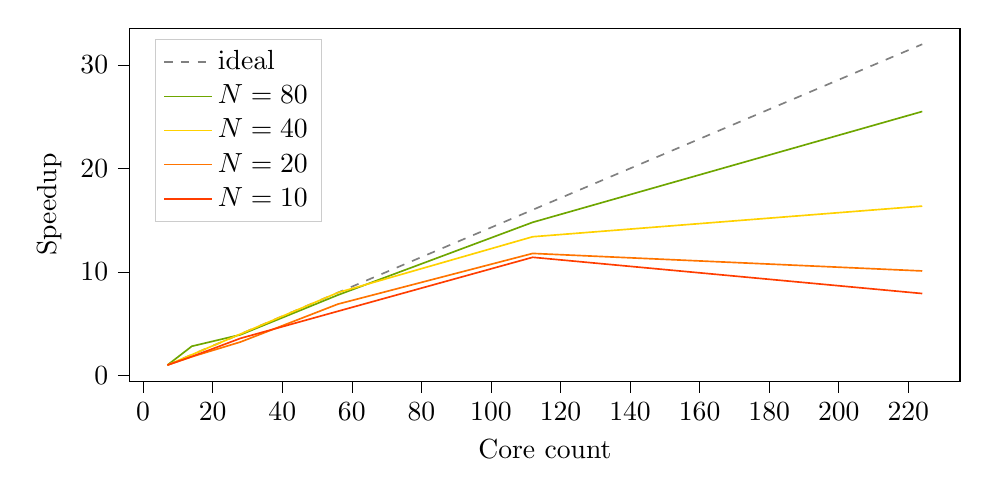
\begin{tikzpicture}

\definecolor{color0}{rgb}{0.431372549019608,0.649134948096886,0}
\definecolor{color1}{rgb}{1,0.81999231064975,0}
\definecolor{color2}{rgb}{1,0.456286043829296,0}
\definecolor{color3}{rgb}{1,0.238062283737024,0}

\begin{axis}[
height=0.5\textwidth,
legend cell align={left},
legend style={fill opacity=0.8, draw opacity=1, text opacity=1, at={(0.03,0.97)}, anchor=north west, draw=white!80!black},
tick align=outside,
tick pos=left,
width=\textwidth,
x grid style={white!69.0196078431373!black},
xlabel={Core count},
xmin=-3.85, xmax=234.85,
xtick style={color=black},
y grid style={white!69.0196078431373!black},
ylabel={Speedup},
ymin=-0.55, ymax=33.55,
ytick style={color=black}
]
\addplot [semithick, white!50.1960784313725!black, dashed]
table {%
7 1
14 2
28 4
56 8
112 16
224 32
};
\addlegendentry{ideal}
\addplot [semithick, color0]
table {%
7 1
14 2.81680077514394
28 3.92854503421451
56 7.76543224645151
112 14.7940949357586
224 25.5032805108307
};
\addlegendentry{$N = 80$}
\addplot [semithick, color1]
table {%
7 1
14 2
28 4
56 8
112 13.3986405956246
224 16.3587854581322
};
\addlegendentry{$N = 40$}
\addplot [semithick, color2]
table {%
7 1
14 1.80134647460197
28 3.22970269035864
56 6.88864405993413
112 11.7860629390055
224 10.091984097319
};
\addlegendentry{$N = 20$}
\addplot [semithick, color3]
table {%
7 1
14 1.81797073276095
28 3.5819768060432
56 6.19790132547864
112 11.4125423728814
224 7.91047932330827
};
\addlegendentry{$N = 10$}
\end{axis}

\end{tikzpicture}

    \caption{Speedup of the equation solver for different proplem sizes $N$.}
    \label{fig:SpeedupEvolution}
\end{figure}


\clearpage

\begin{figure}[p]
    \begin{subfigure}[b]{0.5\textwidth}
        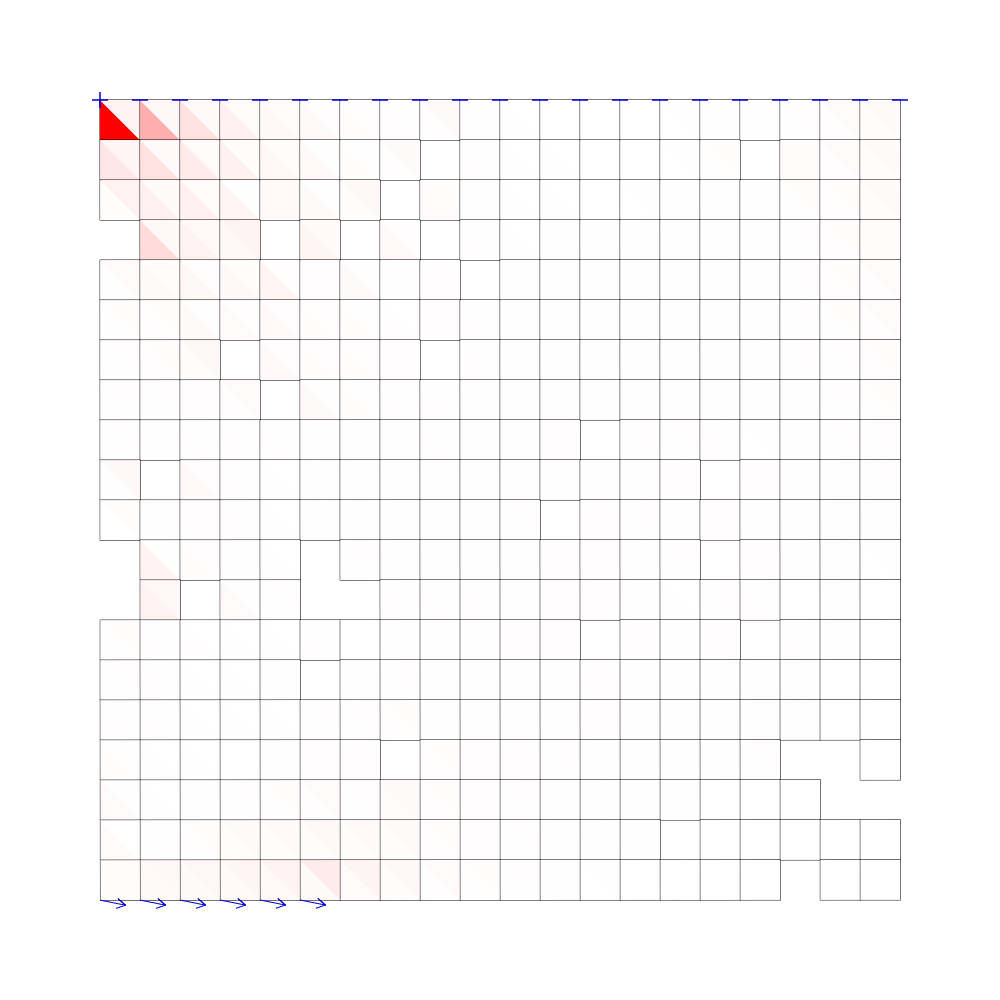
\includegraphics[width=\linewidth]{images/debug0.png} 
    \end{subfigure}%
    \begin{subfigure}[b]{0.5\textwidth}
        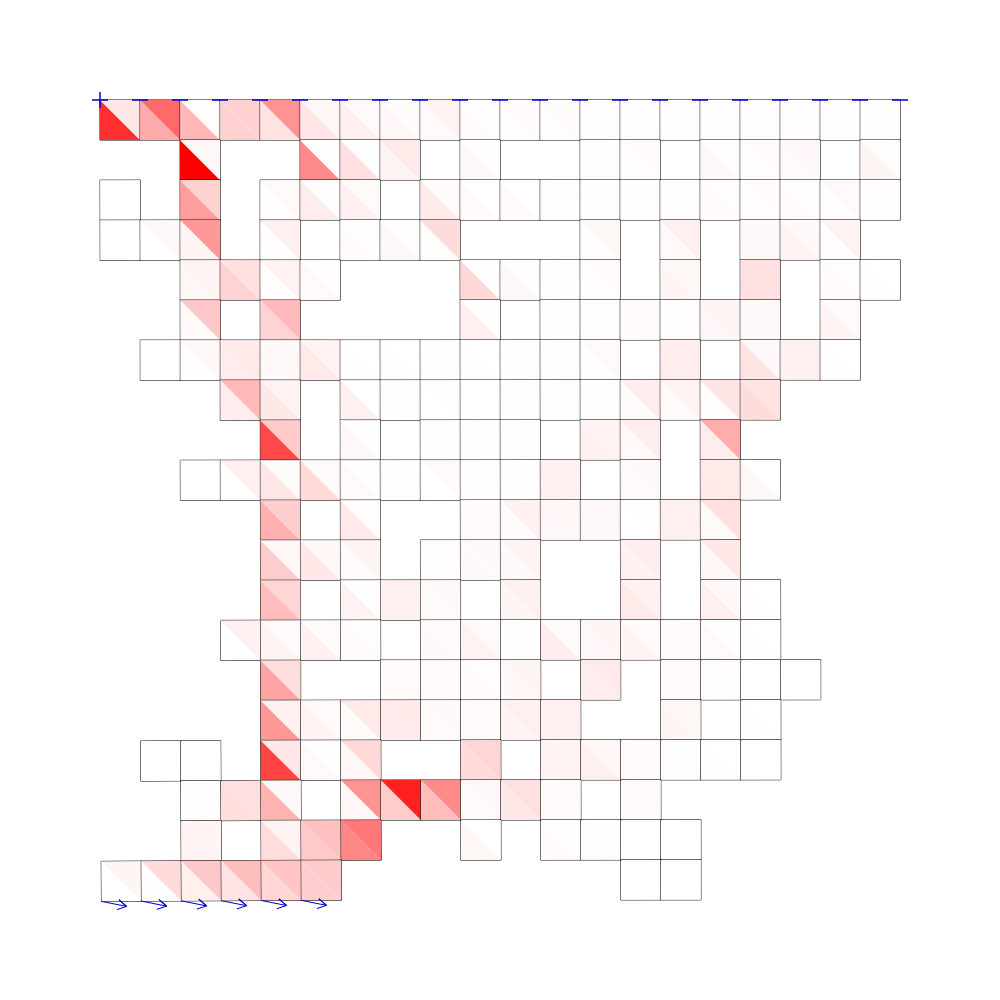
\includegraphics[width=\linewidth]{images/debug900.png} 
    \end{subfigure}

    \begin{subfigure}[b]{0.5\textwidth}
        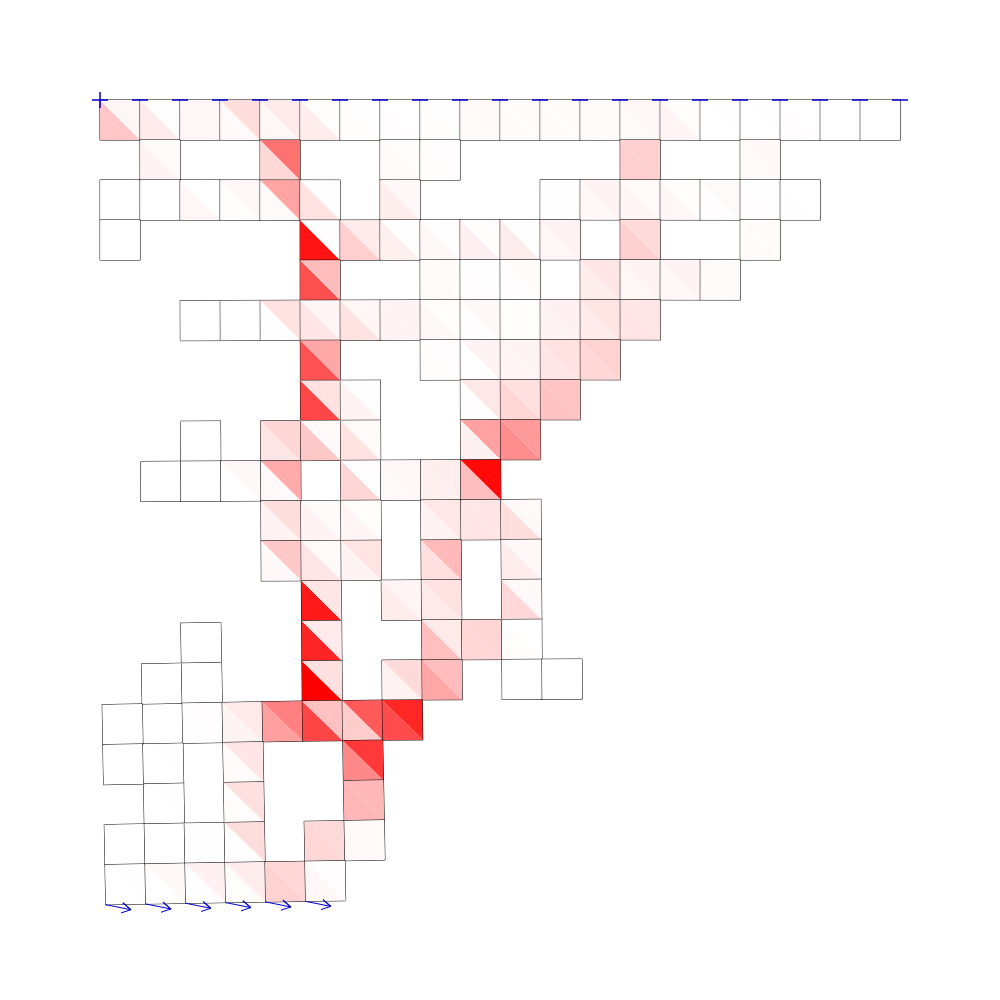
\includegraphics[width=\linewidth]{images/debug1500.png} 
    \end{subfigure}%
    \begin{subfigure}[b]{0.5\textwidth}
        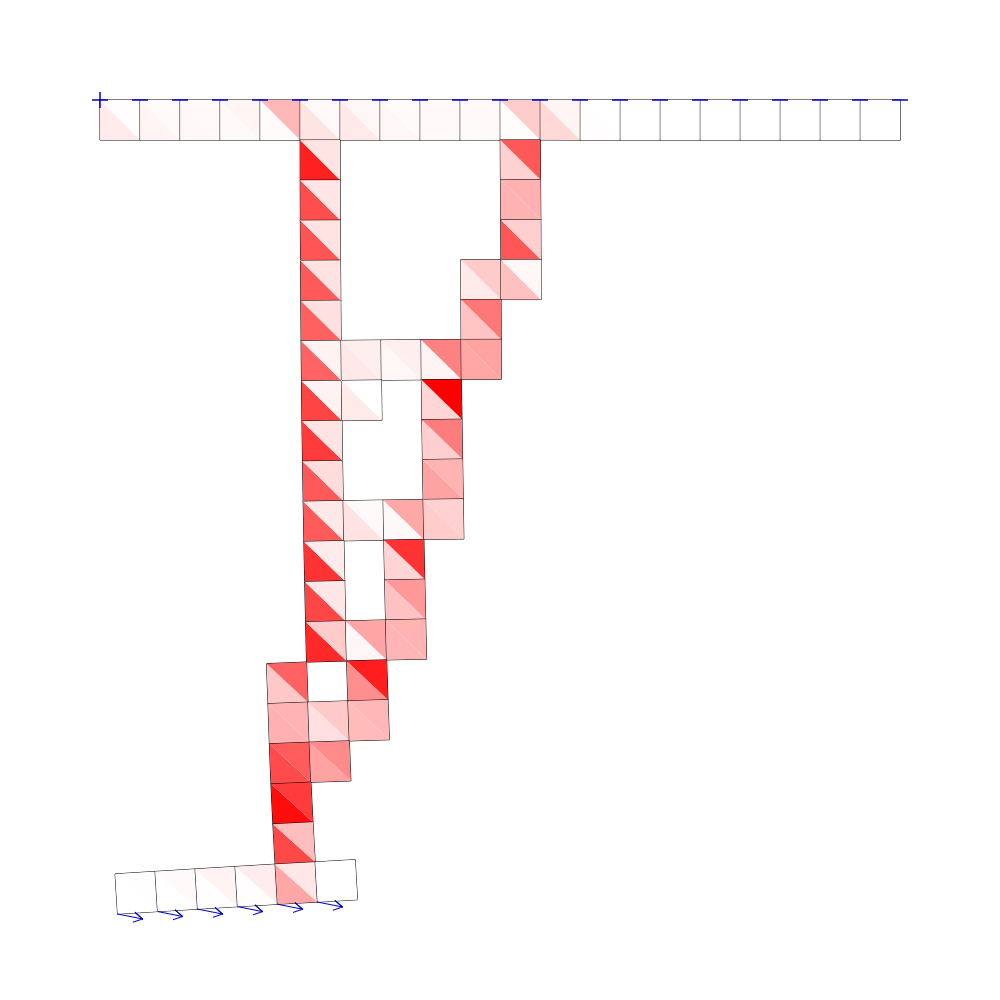
\includegraphics[width=\linewidth]{images/debug8625.png} 
    \end{subfigure}
    \caption{Result of a evoultion, using $20\times20$ gird, 100 organisms per epoch, 1000 epochs and a alterations decay of 0.995. Note, how the structure gets wider on the top to deal with the increased bending stress.}
    \label{fig:Evolution}
\end{figure}


\end{document}